\apendice{Documentación de usuario}

\section{Introducción}

En este apartado se mostrarán los requisitos necesarios para instalar la aplicación así cómo un detallado manual en el que se explica cómo funciona la aplicación. 

\section{Requisitos de usuarios}

El usuario, para poder ejecutar la aplicación ha de poseer un equipo con sistema operativo Windows 10 y una máquina virtual con un sistema operativo Ubuntu-server.

\section{Instalación}

\subsection{\nombrePrograma}
Para instalar \nombrePrograma es necesario tener descargados y almacenados en un mismo directorio del servidor ubuntu los ficheros \textit{install.sh} y el paquete \textit{Monitorizacion\_IOT\_1.0\_all.deb}

Para instalarlo tan solo es necesario ejecutar el siguiente comando:

\begin{lstlisting}[frame=single]  
sudo bash install.sh
\end{lstlisting}

\subsection{PRTG}
Para la instalación de PRTG en un sistema operativo Windows 10 se ha de descargar el programa de la página principal \url{https://www.paessler.com/es/prtg}. La instalación es sencilla y tras acceder al programa se pedirá introducir el usuario y la contraseña, por defecto es \textit{prtgadmin} para ambas, tanto la contraseña cómo el usuario se podrá cambiar.

PRTG por defecto viene ya con una serie de sensores configurados \ref{img_prtg_dispositivos}, los cuales miden parámetros dentro del sistema.

\begin{figure}[h]
	\centering
	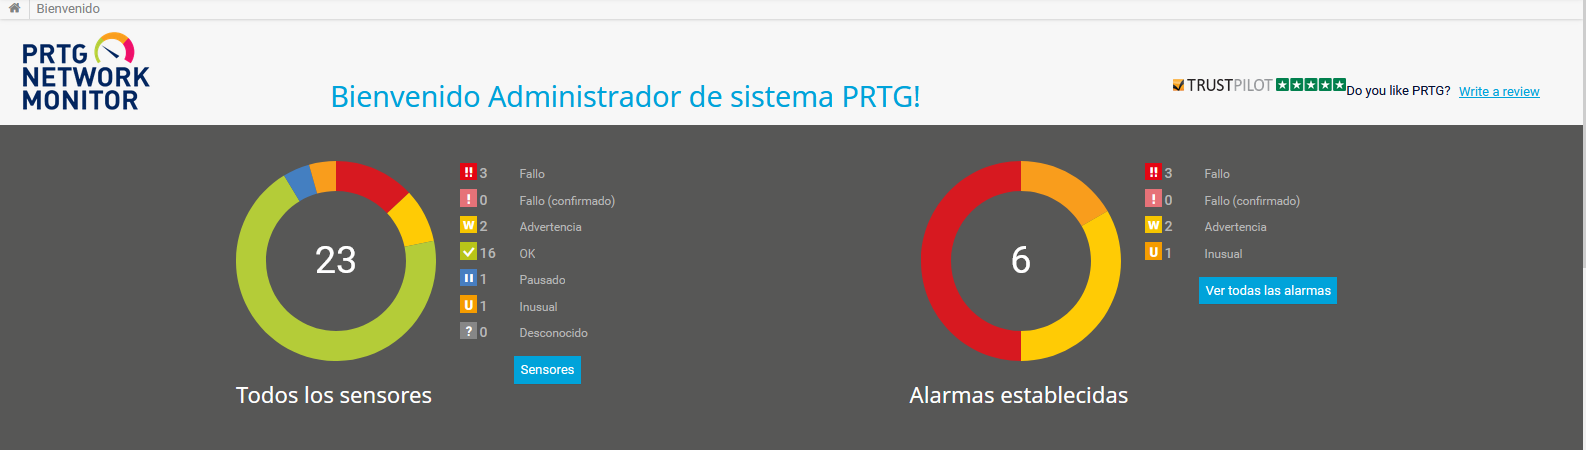
\includegraphics[width=1.1\textwidth]{img/img_prtg_inicio.png}
	\caption{inicio PRTG}
	\label{img_prtg_inicio}
\end{figure}

\begin{figure}[h]
	\centering
	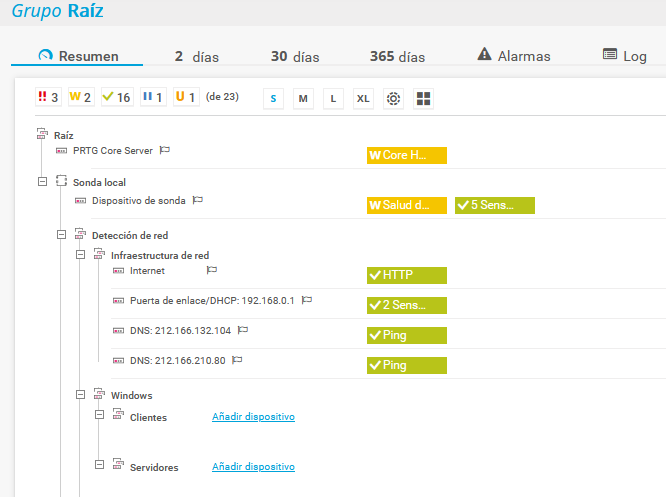
\includegraphics[width=1.1\textwidth]{img/img_prtg_dispositivos.png}
	\caption{dispositivos PRTG}
	\label{img_prtg_dispositivos}
\end{figure}

\begin{figure}[h]
	\centering
	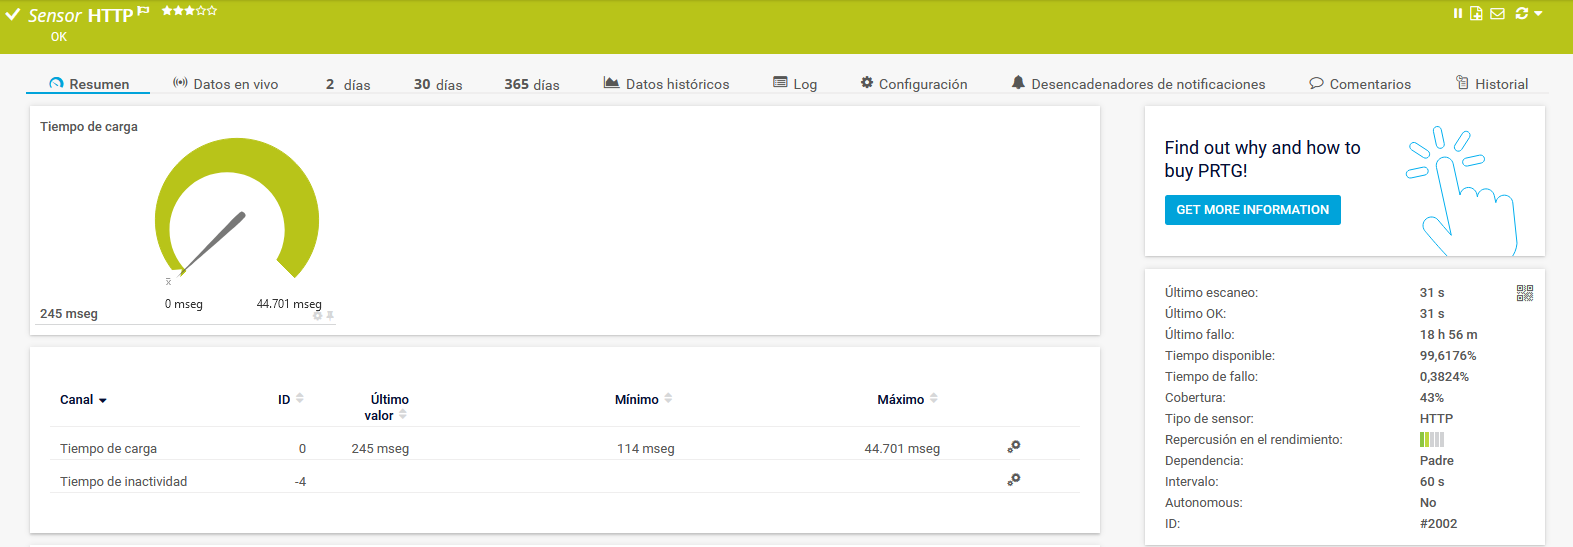
\includegraphics[width=1.1\textwidth]{img/img_ejemplo sensor.png}
	\caption{ejemplo sensor PRTG}
	\label{img_ejemplo}
\end{figure}

\clearpage

\section{Manual del usuario}

Este apartado pretende hacer de guía al usuario a través de la aplicación, mostrando cómo funciona el sistema y cómo es posible configurarlo.

\subsection{Configuración}

 Una vez se haya instalado \nombrePrograma hay una serie de modificaciones que hay que realizar manualmente antes de poder ser ejecutado.
 
\subsubsection{Logstash}

 El primero sería en el fichero del logstash, el cual se encuentra en la ruta: \textit{/etc/logstash/conf.d/logstashSensor.conf}
 
 En él se encuentra el mecanismo que permite a logstash procesar los archivos de logs con los datos de los sensores y enviárselos a la BBDD de Elasticsearch.
 
 \begin{verbatim}
input{
        http{
                id=> "sensor_data_http_input"
        }
}

filter{

        ruby {
                code => '
                    event.get("reading").each { |k, v|
                        event.set(k,v)
                    }
                    event.remove("reading")
                '
            }

}
output{

        elasticsearch{
                hosts => ["localhost:9200", "IP_Ubuntu_server:9200"]
                index => "sensor_data-%{+YYYY.MM.dd}"
        }
}
 \end{verbatim}
 
Para que logstash mande la información a Elasticsearch hay que sustituir donde pone ``IP\_Ubuntu\_server'' por la IP de Ubuntu server, en el cual se ha instalado Elasticsearch.

\subsubsection{Índice}

Logstash ahora ya sabe a dónde enviar los datos, pero se ha de preparar Elasticsearch para su llegada, se ha de crear un índice que diga a Elasticsearch que datos esperar.

Para ello se ha de acceder a la página principal de Elastic, introduciendo en un navegador web del host la url: \textit{IP\_Ubuntu\_server:5601}, donde \textit{IP\_Ubuntu\_server} es la ip del servidor.

Una vez se haya accedido a Elastic, para crear un índice se ha de acceder a \textit{Dev Tools}, accediendo desde el menú desplegable izquierdo, en el apartado de \textit{Management} se ha de introducir el POST con el índice \ref{indice} y enviar la \textit{request} cómo se puede observar en la figura \ref{img_index}



\begin{listing}
\begin{minted}[frame=single,
               framesep=3mm,
               linenos=true,
               xleftmargin=21pt,
               tabsize=6]{js}

POST _template/sensor_data_template
{
  "index_patterns": [
    "sensor_data*"
  ],
  "settings": {
    "number_of_replicas": "1",
    "number_of_shards": "5"
  },
  "mappings": {
    "properties": {
      "sensorId": {
        "type": "integer"
      },
      "datetime":{
        "type": "date",
        "format": "dd/MM/yyyy HH:mm:ss"
      },
      "reading": {
        "type": "nested", 
        "properties": { 
          "name": {"type":"keyword"},
          "description": {"type":"double"}
        }
      }
    }
  }
}


\end{minted}
\caption{Índice} 
\label{indice}
\end{listing}

\begin{figure}[h]
	\centering
	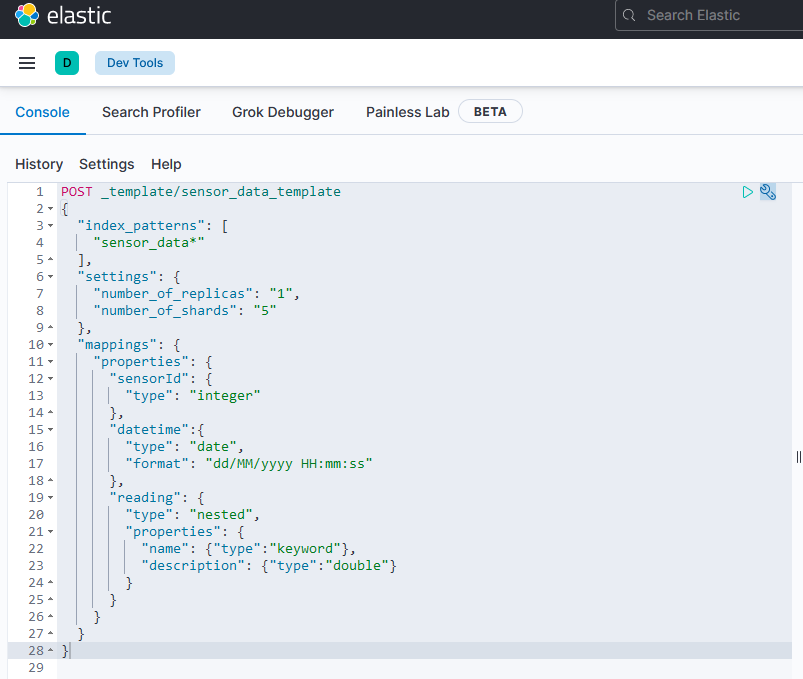
\includegraphics[width=1.1\textwidth]{img/img_crear_patron.png}
	\caption{Crear un índice}
	\label{img_index}
\end{figure}
\newpage

Una vez creado el índice todos los datos procedentes de losgstash se almacenarán con ese índice.
Dentro del menú \textit{Stack Management} en el apartado \textit{index Managment} se puede consultar los datos que va recibiendo \ref{img_index_manager.png}.

\begin{figure}[h]
	\centering
	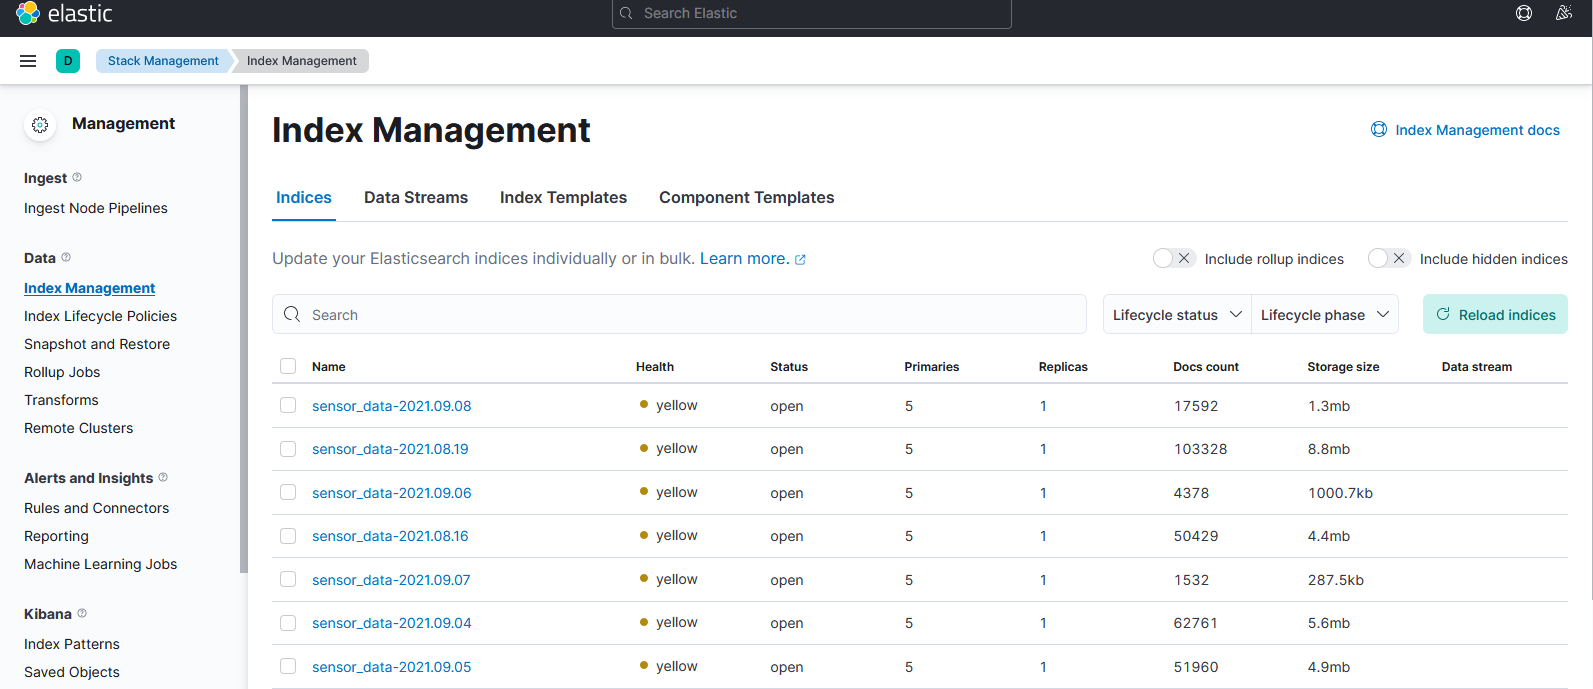
\includegraphics[width=1.1\textwidth]{img/img_index_manager.png}
	\caption{Index Managment}
	\label{img_index_manager.png}
\end{figure}

\newpage

\subsection{configuración de parámetros}

El usuario puede elegir que sensores desea almacenar y entrenar así cómo cada cuanto tiempo se desea ejecutar el programa y seleccionar cuantos instantes de tiempo en el futuro se desea predecir. Para ello se ha de acceder al fichero \textit{/usr/bin/Monitorizacion\_IOT/Monitorizacion\_IOT.sh} en él, se encintarán una serie de variables que el usuario ha de modificar.

\begin{itemize}
    \item \textbf{usuario\_PRTG}: se ha de introducir el nombre de usuario de PRTG
    \item \textbf{passhash\_PRTG}: se ha de introducir el passhash de PRTG
    \item \textbf{lista\_id\_sensor}: en esta lista se ha de introducir el id de los sensores, separados por un espacio.
    \item \textbf{horizonte\_predicción}: se ha de introducir cuantos minutos a futuro se desea que llegue la predicción.
    \item \textbf{repeticion\_ciclo}: Se ha de introducir el tiempo en segundos que ha de esperar el sistema entre ciclo y ciclo. 
\end{itemize}

Para saber la dirección IP de PRTG hay que acceder, dentro de PRTG a configuración > interfaz de usuario > combinaciones de puertos / servidor web direcciones IP activas y para saber el passhash se ha de acceder a configuración > mi cuenta > Configuración de cuenta de usuario y mostrar passhash.

\subsection{Crear un modelo para los sensores}

Para la realización del entrenamiento sobre los datos procedentes de un sensor, es esencial crear y configurar cada modelo a mano, respondiendo a las necesidades de estos.

Para crear un modelo hay que modificar de forma manual el fichero \textit{/usr/bin/Monitorizacion-IOT/Prediccion/Crear\_modelo.py}, una vez en el fichero, se ha de generar una instancia del modelo que se dese crear pasando cómo parámetro el id del sensor. A continuación, llamaremos a la función inicializar del modelo, pasándole los parámetros necesarios. Por último se llama al método guardar de la clase \textit{Persistencia\_modelo}. Para guardar el modelo simplemente compilamos el fichero, este se guardará en la carpeta \textit{/usr/bin/Monitorizacion-IOT/Prediccion/modelos/} y se podrá usar para el entrenamiento y la predicción.

\begin{verbatim}
if __name__ == "__main__":

    idSensor = 4051

    modelo = Modelo_SNARIMAX(idSensor)
    modelo.inicializar(q=2,
                        m=30,
                        sp=6,
                        sq=10,
                        intercept_init=12,
                        sgd=0.01, 
                        intercerpt_lr=0.3)

    Persistencia_modelo.guardar(modelo)

\end{verbatim}

\subsection{Inicialización y parada del sistema}

Una vez configurado el programa se puede inicializar y poner en marcha todo el sistema, para ello se ha de introducir el siguiente comando:

\begin{lstlisting}[frame=single]  
systemctl start Monitorizacion_IOT
\end{lstlisting}

para realizar la parada completa del sistema y que este deje de captar datos de PRTG se ha de introducir el siguiente comando:

\begin{lstlisting}[frame=single]  
systemctl stop Monitorizacion_IOT
\end{lstlisting}


\subsection{Index pattern}

Por último, para poder explorar y visualizar los datos en Kibana es necesarios que exista un ``index pattern'' que diga a Elasticsearch que índices contienen los datos, así como especificar de que tipo son. \cite{pagina:elastic}

Para poder crear un index pattern, primero Elasticsearch ha de tener datos \ref{img_index_pattern_antes_de_datos.png}, es por ello que este es el último paso a realizar.

Una vez se disponga de datos se podrá crear un index pattern \ref{img_index_patter_menu.png}

En este caso se ha de crear un patrón para que albergue todos los datos procedentes de sensores ``sensor\_data-*'' \ref{img_create_index_pattern.png}

\begin{figure}[h]
	\centering
	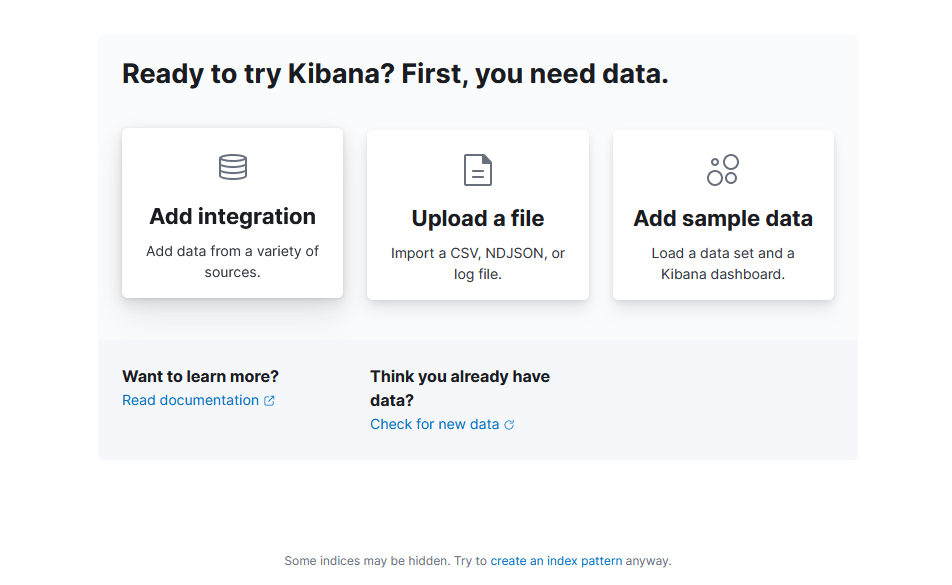
\includegraphics[width=1.1\textwidth]{img/img_index_pattern_antes_de_datos.png}
	\caption{Index pattern menú inicial si no se encuentran datos en Elasticsearch}
	\label{img_index_pattern_antes_de_datos.png}
\end{figure}

\begin{figure}[h]
	\centering
	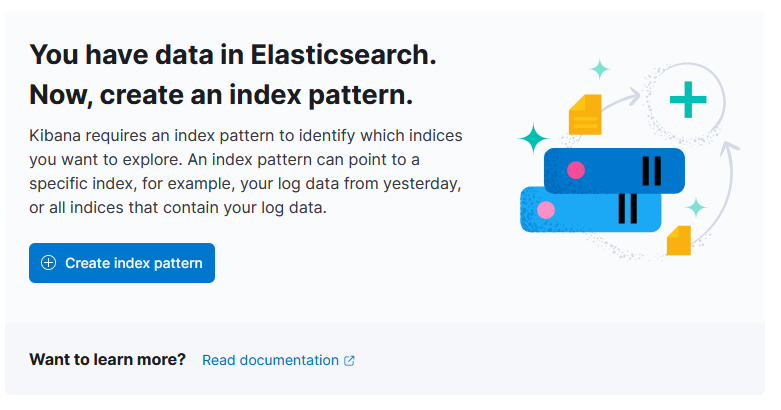
\includegraphics[width=1.1\textwidth]{img/img_index_patter_menu.png}
	\caption{Index pattern menú inicial}
	\label{img_index_patter_menu.png}
\end{figure}

\begin{figure}[h]
	\centering
	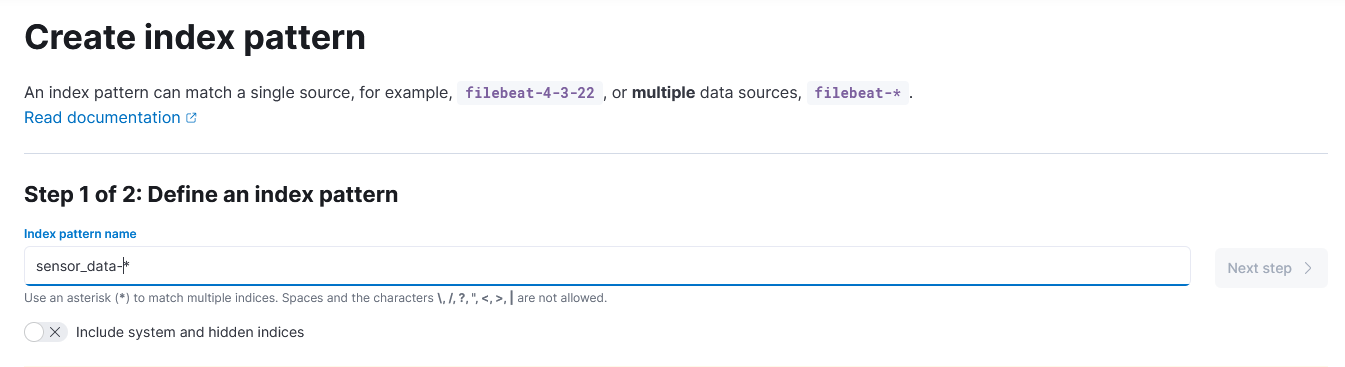
\includegraphics[width=1.1\textwidth]{img/img_create_index_pattern.png}
	\caption{Creación de un index pattern}
	\label{img_create_index_pattern.png}
\end{figure}

Una vez creado el patrón se pedirá que se configure, se puede especificar cuál va a ser el índice de los datos, si el tiempo en el que es indexado a en Elasticsearch ``@timestamp'' u otro campo fecha que se prefiera. \ref{img_conf_index_pattern.png}

También se puede cambiar el tipo de cualquier otro campo. 

\begin{figure}[h]
	\centering
	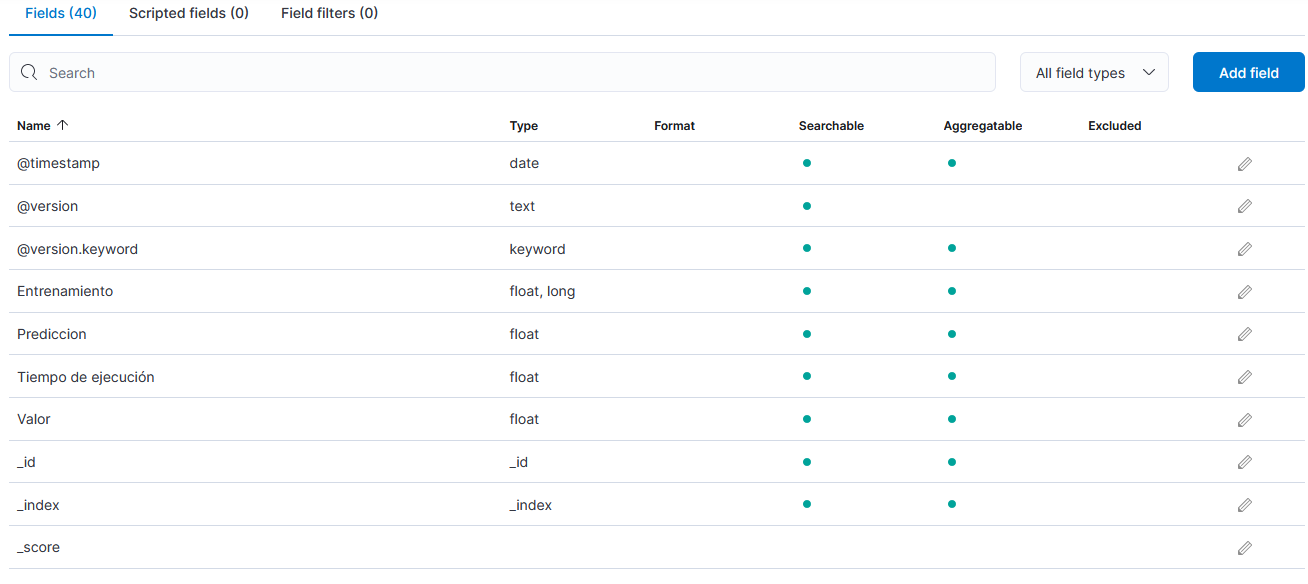
\includegraphics[width=1.1\textwidth]{img/img_conf_index_pattern.png}
	\caption{Configuración de un index pattern}
	\label{img_conf_index_pattern.png}
\end{figure}

\clearpage

\subsection{¿Cómo funciona \nombrePrograma?}

Una vez configurado e inicializado, el programa captará los datos de los sensores, los entrenará y realizará las predicciones. A continuación, se explicarán que proceses sigue. 

\nombrePrograma es un programa que se repite en bucle, cada ciclo se repite cada x tiempo, dependiendo del valor de la variable \textit{repeticion\_ciclo}. En cada ciclo se descargan, se entrenan y se predicen los datos de cada sensor. 

\subsubsection{Obtención y almacenamiento de datos}\label{cap:obt_alm_datos}

Para poder trabajar con los datos de los sensores, provenientes de PRTG es necesario descargarlos y almacenarlos para poder realizar el estudio y entrenamiento de dichos datos.

\nombrePrograma, mediante un script, descarga los datos de los sensores que se encuentran en la lista \textbf{lista\_id\_sensor}, estos se guardan en un fichero JSON, el cual se ha de transformar para adecuar el formato y que Elasticsearch pueda procesarlo. Para almacenar los datos ya obtenidos y transformados a la base de datos de Elasticsearch, estos ficheros son preprocesados por logstash que se encarga de enviar las líneas de datos al servidor de Elastic e indexarlos correctamente.

Los datos son subidos con el siguiente nombre: ``sensor\_data-yyyy.mm.dd'' de tal forma que todos los datos que se suben en un día se almacenan bajo un mismo índice. Para poder explorar y visualizar los datos en Kibana es necesarios que exista un ``index pattern'' que diga a Elasticsearch que índices contienen los datos, así como especificar de que tipo son, en este caso se ha creado uno para que albergue todos los datos procedentes de sensores ``sensor\_data-*''. 

Una vez los datos estén correctamente almacenados e indexados en Elasticsearch, se puede explorar y visualizar los datos con Kibana.


\newpage
\subsubsection{Transformación de datos}\label{cap:TransformacionDatos}

Durante la transformación de los ficheros JSON se eliminan los datos irrelevantes que se obtenían de PRTG, se añade el id del sensor y se cambia el formato de la fecha de dd/MM/yyyy H:mm:ss a dd/MM/yyyy HH:mm:ss.

Logstash esta preparado para trabajar con logs, es por eso que además también se separa cada entrada de datos por líneas, cómo se puede observar el los Listings \ref{json-example} y \ref{json-transformado-example}

\begin{listing}
\begin{minted}[frame=single,
               framesep=3mm,
               linenos=true,
               xleftmargin=21pt,
               tabsize=6]{js}
{
    "prtg-version":"21.2.68.1492",
    "treesize":30,
    "histdata":
    [
        {
            "datetime":"27/07/2021 16:11:06",
            "Valor":4.6800,
            "Tiempo de ejecución":782.0000,
            "coverage":"100 %"
        },
        {
            "datetime":"27/07/2021 16:12:06",
            "Valor":4.6800,
            "Tiempo de ejecución":797.0000,
            "coverage":"100 %"
        },
        {
            "datetime":"27/07/2021 16:13:06",
            "Valor":4.6700,
            "Tiempo de ejecución":799.0000,
            "coverage":"100 %"
        }
    ]
}

\end{minted}
\caption{JSON descargado de PRTG} 
\label{json-example}
\end{listing}

\begin{listing}
\begin{minted}[frame=single,
               framesep=3mm,
               linenos=true,
               xleftmargin=21pt,
               tabsize=6]{js}

{
    "sensorId":"2051",
    "datetime":"27/07/2021 16:11:06",
    "reading": 
    {
        "Valor":4.6800,
        "Tiempo de ejecución":782.0000
    }
}
{
    "sensorId":"2051",
    "datetime":"27/07/2021 16:12:06",
    "reading": 
    {
        "Valor":4.6800,
        "Tiempo de ejecución":797.0000
    }
}
{
    "sensorId":"2051",
    "datetime":"27/07/2021 16:13:06",
    "reading": 
    {
        "Valor":4.6700,
        "Tiempo de ejecución":799.0000
    }
}

\end{minted}
\caption{JSON transformado} 
\label{json-transformado-example}
\end{listing}

\newpage



\subsubsection{Machine learning}

\textbf{Incremental/Online Learning}

Cómo se ha especificado en el apartado de conceptos teóricos el incremental learning va entrenando el modelo con datos en un flujo continuo. Esto es muy beneficioso ya que en este proyecto en concreto no se dispone de muestras lo suficientemente grandes como para entrenar un modelo mediante la forma tradicional de \textit{batch learning} de forma eficaz. 

\textbf{Entrenamiento}

Una vez los datos de los sensores están correctamente indexados y almacenados en Elasticsearch se puede proceder al entrenamiento.

Por cada sensor se cargará el modelo que se haya creado para ese modelo en concreto y se descargarán los datos en un rango de fecha determinado desde Elasticsearch. Los valores de entrenamiento serán volcados a un fichero y devueltos a Elasticsearch, para poder monitorizar el entrenamiento.

Una vez se ha finalizado se guarda el modelo en disco para que la siguiente vez que se requiera entrenar modelo o hacer predicciones se utilice siempre el modelo más actualizado.

\textbf{Predicción}

Cada ciclo del programa se hace una predicción de los siguientes minutos (según se indique en la variable \textit{horizonte\_prediccion}), para no acumular datos repetidos en la BBDD, se eliminan los datos que se han predicho en el ciclo anterior. Así cada predicción que hace el programa esta actualizada.

Esta predicción se sube a Elasticsearch para poder ser visualizada.

\begin{figure}[h]
	\centering
	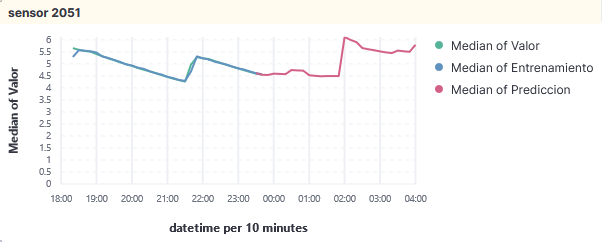
\includegraphics[width=1.1\textwidth]{img/img_prediccion_sensor2051.png}
	\caption{predicción sensor de Presión Tubería de Agua}
	\label{img_prediccion_sensor2051}
\end{figure}
\newpage


\subsection{Visualización y monitorización}

Mediante un navegador introducimos la siguiente url: IP\_ubuntu\_server:5601 (el puerto 5601 corresponde al de kibana).

\begin{figure}[h]
	\centering
	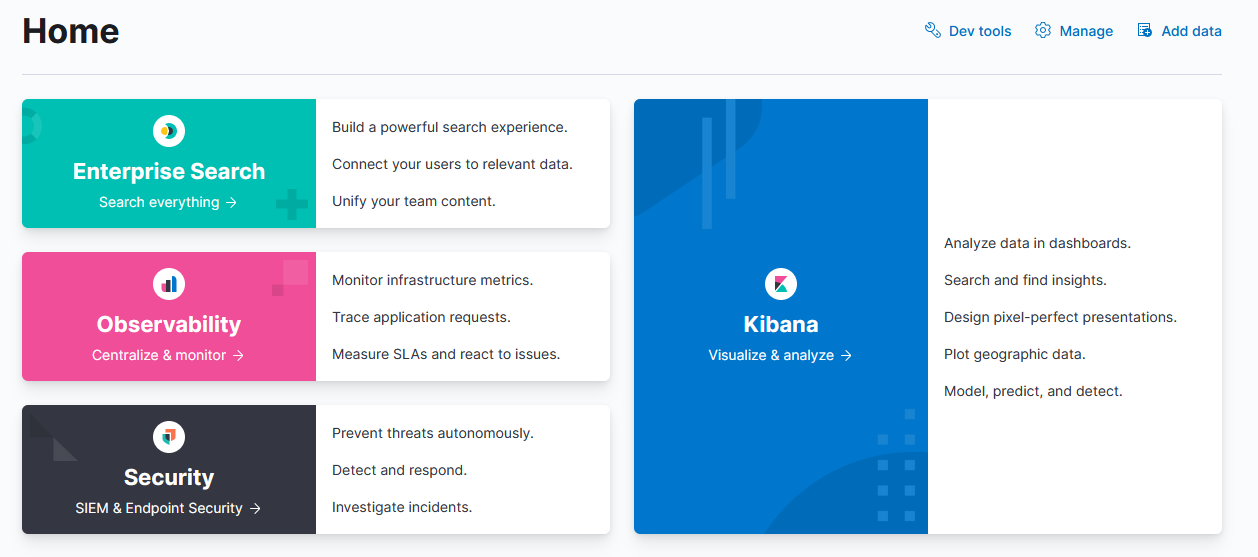
\includegraphics[width=1.1\textwidth]{img/img_kibana_home.png}
	\caption{pagina inicio kibana}
	\label{img_kibana_home}
\end{figure}

Una vez en el apartado home podemos acceder al apartado ``kibana Visualize \& analyze'' para poder echar un vistazo a nuestros datos. Para ver nuestros datos, así como realizar filtrados y búsquedas accederemos a ``Discover''

Se pueden visualizar los datos que estén vinculados a un patrón de índices.

\begin{figure}[h]
	\centering
	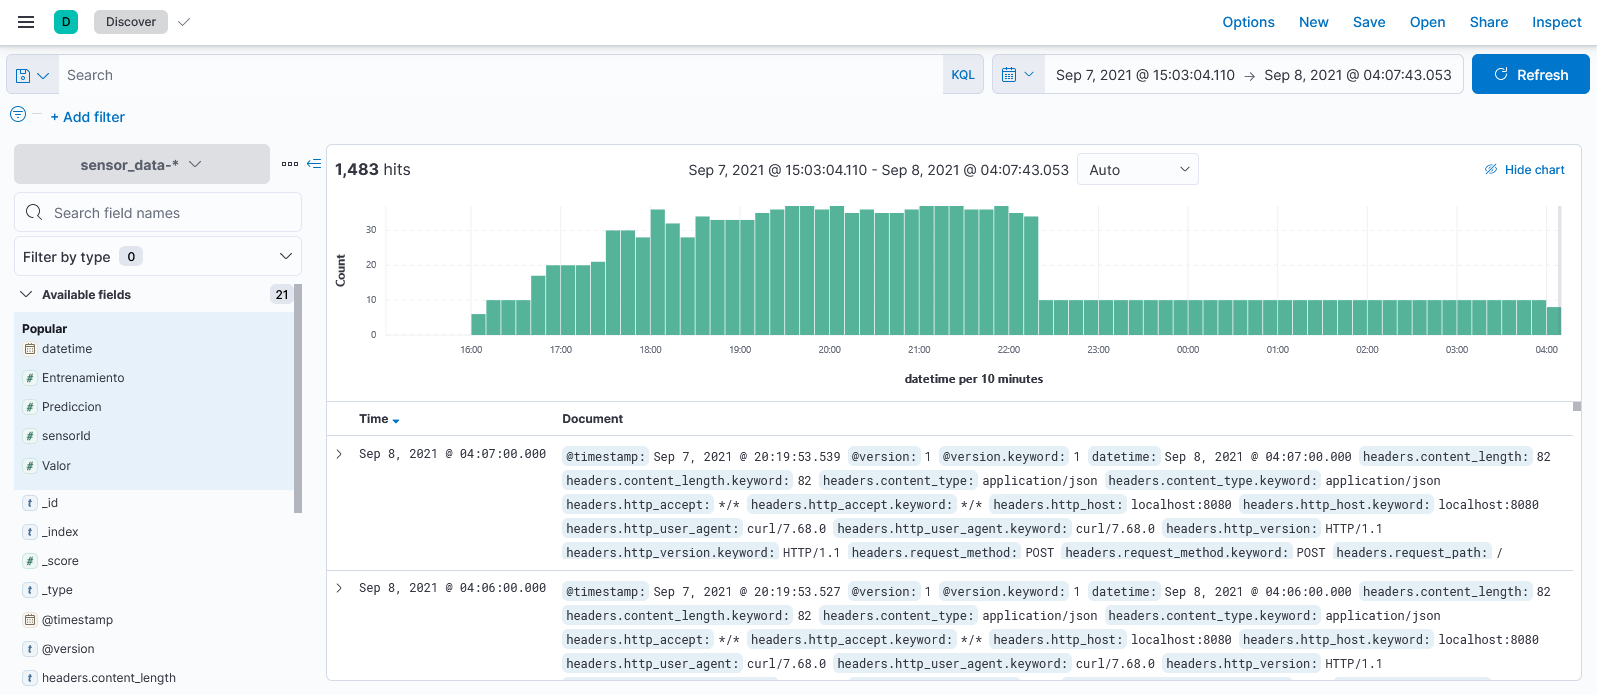
\includegraphics[width=1.1\textwidth]{img/img_kibana_discover.png}
	\caption{kibana discover}
	\label{img_kibana_discover}
\end{figure}

Para visualizar de forma gráfica los datos se ha de acceder al apartado ``Dashboard'' en él se puede crear cualquier tipo de gráfico.

\begin{figure}[h]
	\centering
	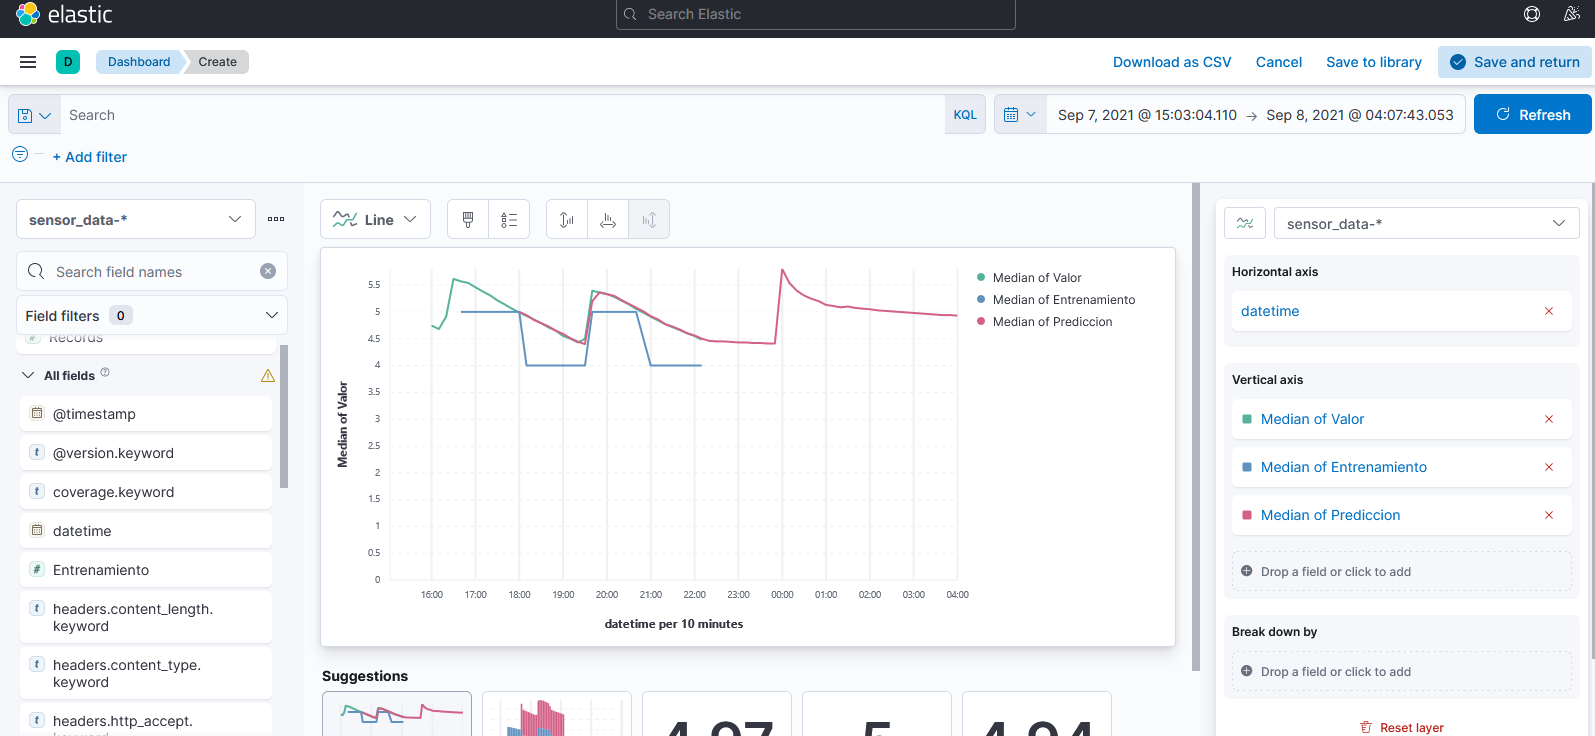
\includegraphics[width=1.1\textwidth]{img/img_kibana_dashboard.png}
	\caption{kibana dashboard}
	\label{img_kibana_dashboard}
\end{figure}


\subsection{Búsquedas y filtrados de datos}

kibana provee varias formas de construir queries con las cuales poder hacer filtrados y búsquedas en los datos almacenados en Elasticsearch.

En el apartado \textit{Discover} se muestran los datos de un índice, se pueden realizar una serie de filtrados y búsquedas, el filtrado de tiempo limita los datos mostrados en un rango de fechas, este filtrado, normalmente, se aplica al campo de tiempo del \textit{intex pattern}

\begin{figure}[h]
	\centering
	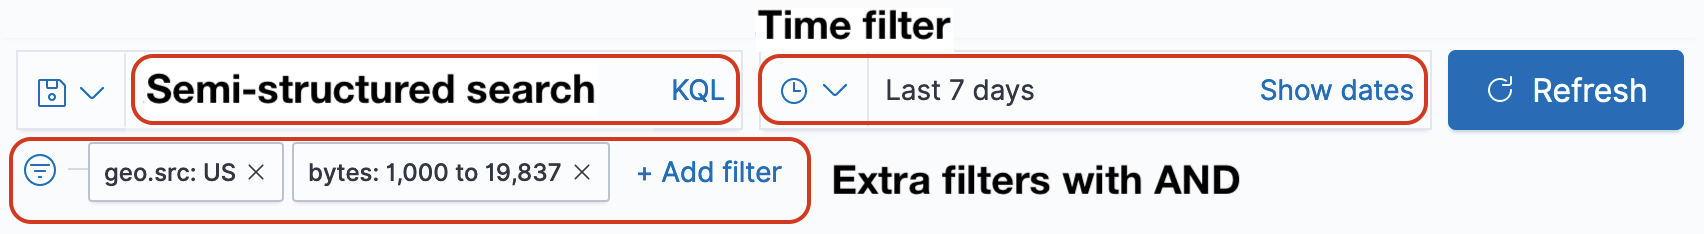
\includegraphics[width=1.1\textwidth]{img/img_time_filter.png}
	\caption{kibana filtrados}
	\label{img_time_filter.png}
\end{figure}

La sintaxis que se utilizada es KQL (Kibana Query Language) un lenguaje creado específicamente para facilitar las búsquedas y filtrados en Elasticsearch. \cite{pagina:KQL}

\begin{figure}[h]
	\centering
	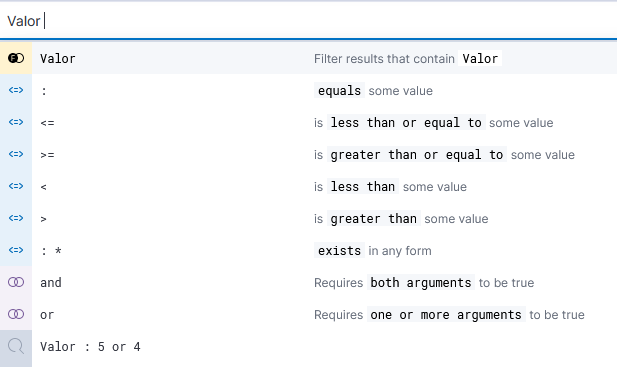
\includegraphics[width=1.1\textwidth]{img/img_fitradoDatos.png}
	\caption{kibana ayuda de filtrado}
	\label{img_fitradoDatos.png}
\end{figure}
